\chapter{PCA - Principal Component Analysis}
PCA is a tool used to find a low dimensional representation of a data set that represent as much variation as the complete data set.   The analysis finds uncorrelated variables named principal components from the dataset.  The first principal component is the one which represent the most variance of the the dataset, and declines.  Each Principal Component are orthogonal with the other ones. 

\begin{figure}[H]
\centering
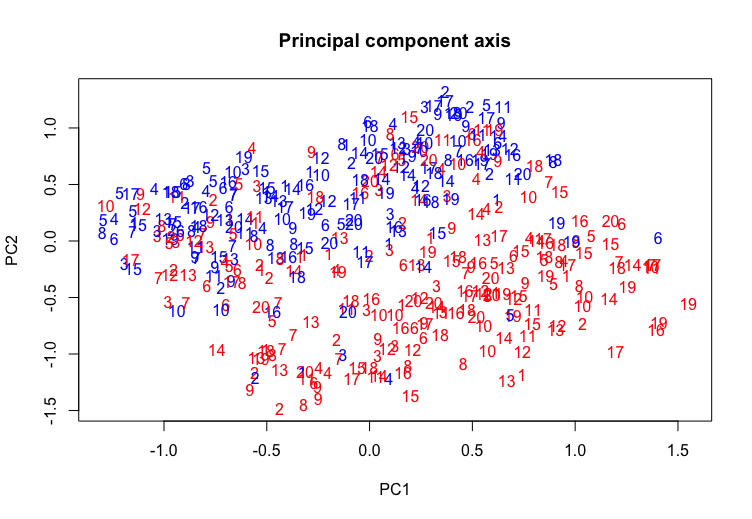
\includegraphics[width = \textwidth]{Figure/PCa-axis.png}
\caption{ red numbers indicated the axis of PC1 and the blue numbers determine the axis of PC2}
\label{fig:pca_vis}
\end{figure}

An illustration of the first two principal components of Person dependent dataset can be seen in figure \ref{fig:pca_vis}.  The red numbers covers mostly the horizontal axis, and the varies mostly in the direction, where as the blue numbers  covers more of the vertical axis than the horizontal axis. 


\missingfigure{PCA plot Independent and dependent}

%\begin{figure}
%\centering
%\begin{subfigure}{.7\textwidth}
%  \centering
%  \includegraphics[width=.4\linewidth]
%  \caption{A subfigure}
%  \label{fig:sub1}
%\end{subfigure}%
%\begin{subfigure}{.5\textwidth}
%  \centering
%  \includegraphics[width=.4\linewidth]
%  \caption{A subfigure}
%  \label{fig:sub2}
%\end{subfigure}
%\caption{A figure with two subfigures}
%\label{fig:test}
%\end{figure}


\begin{figure}
  \hspace*{\fill}%
  \subcaptionbox{2a\label{fig2:a}}{\includegraphics[width=1.7in]{Figure/accumulated-2-1-person-independent.png}}\hfill%
  \subcaptionbox{2b\label{fig2:b}}{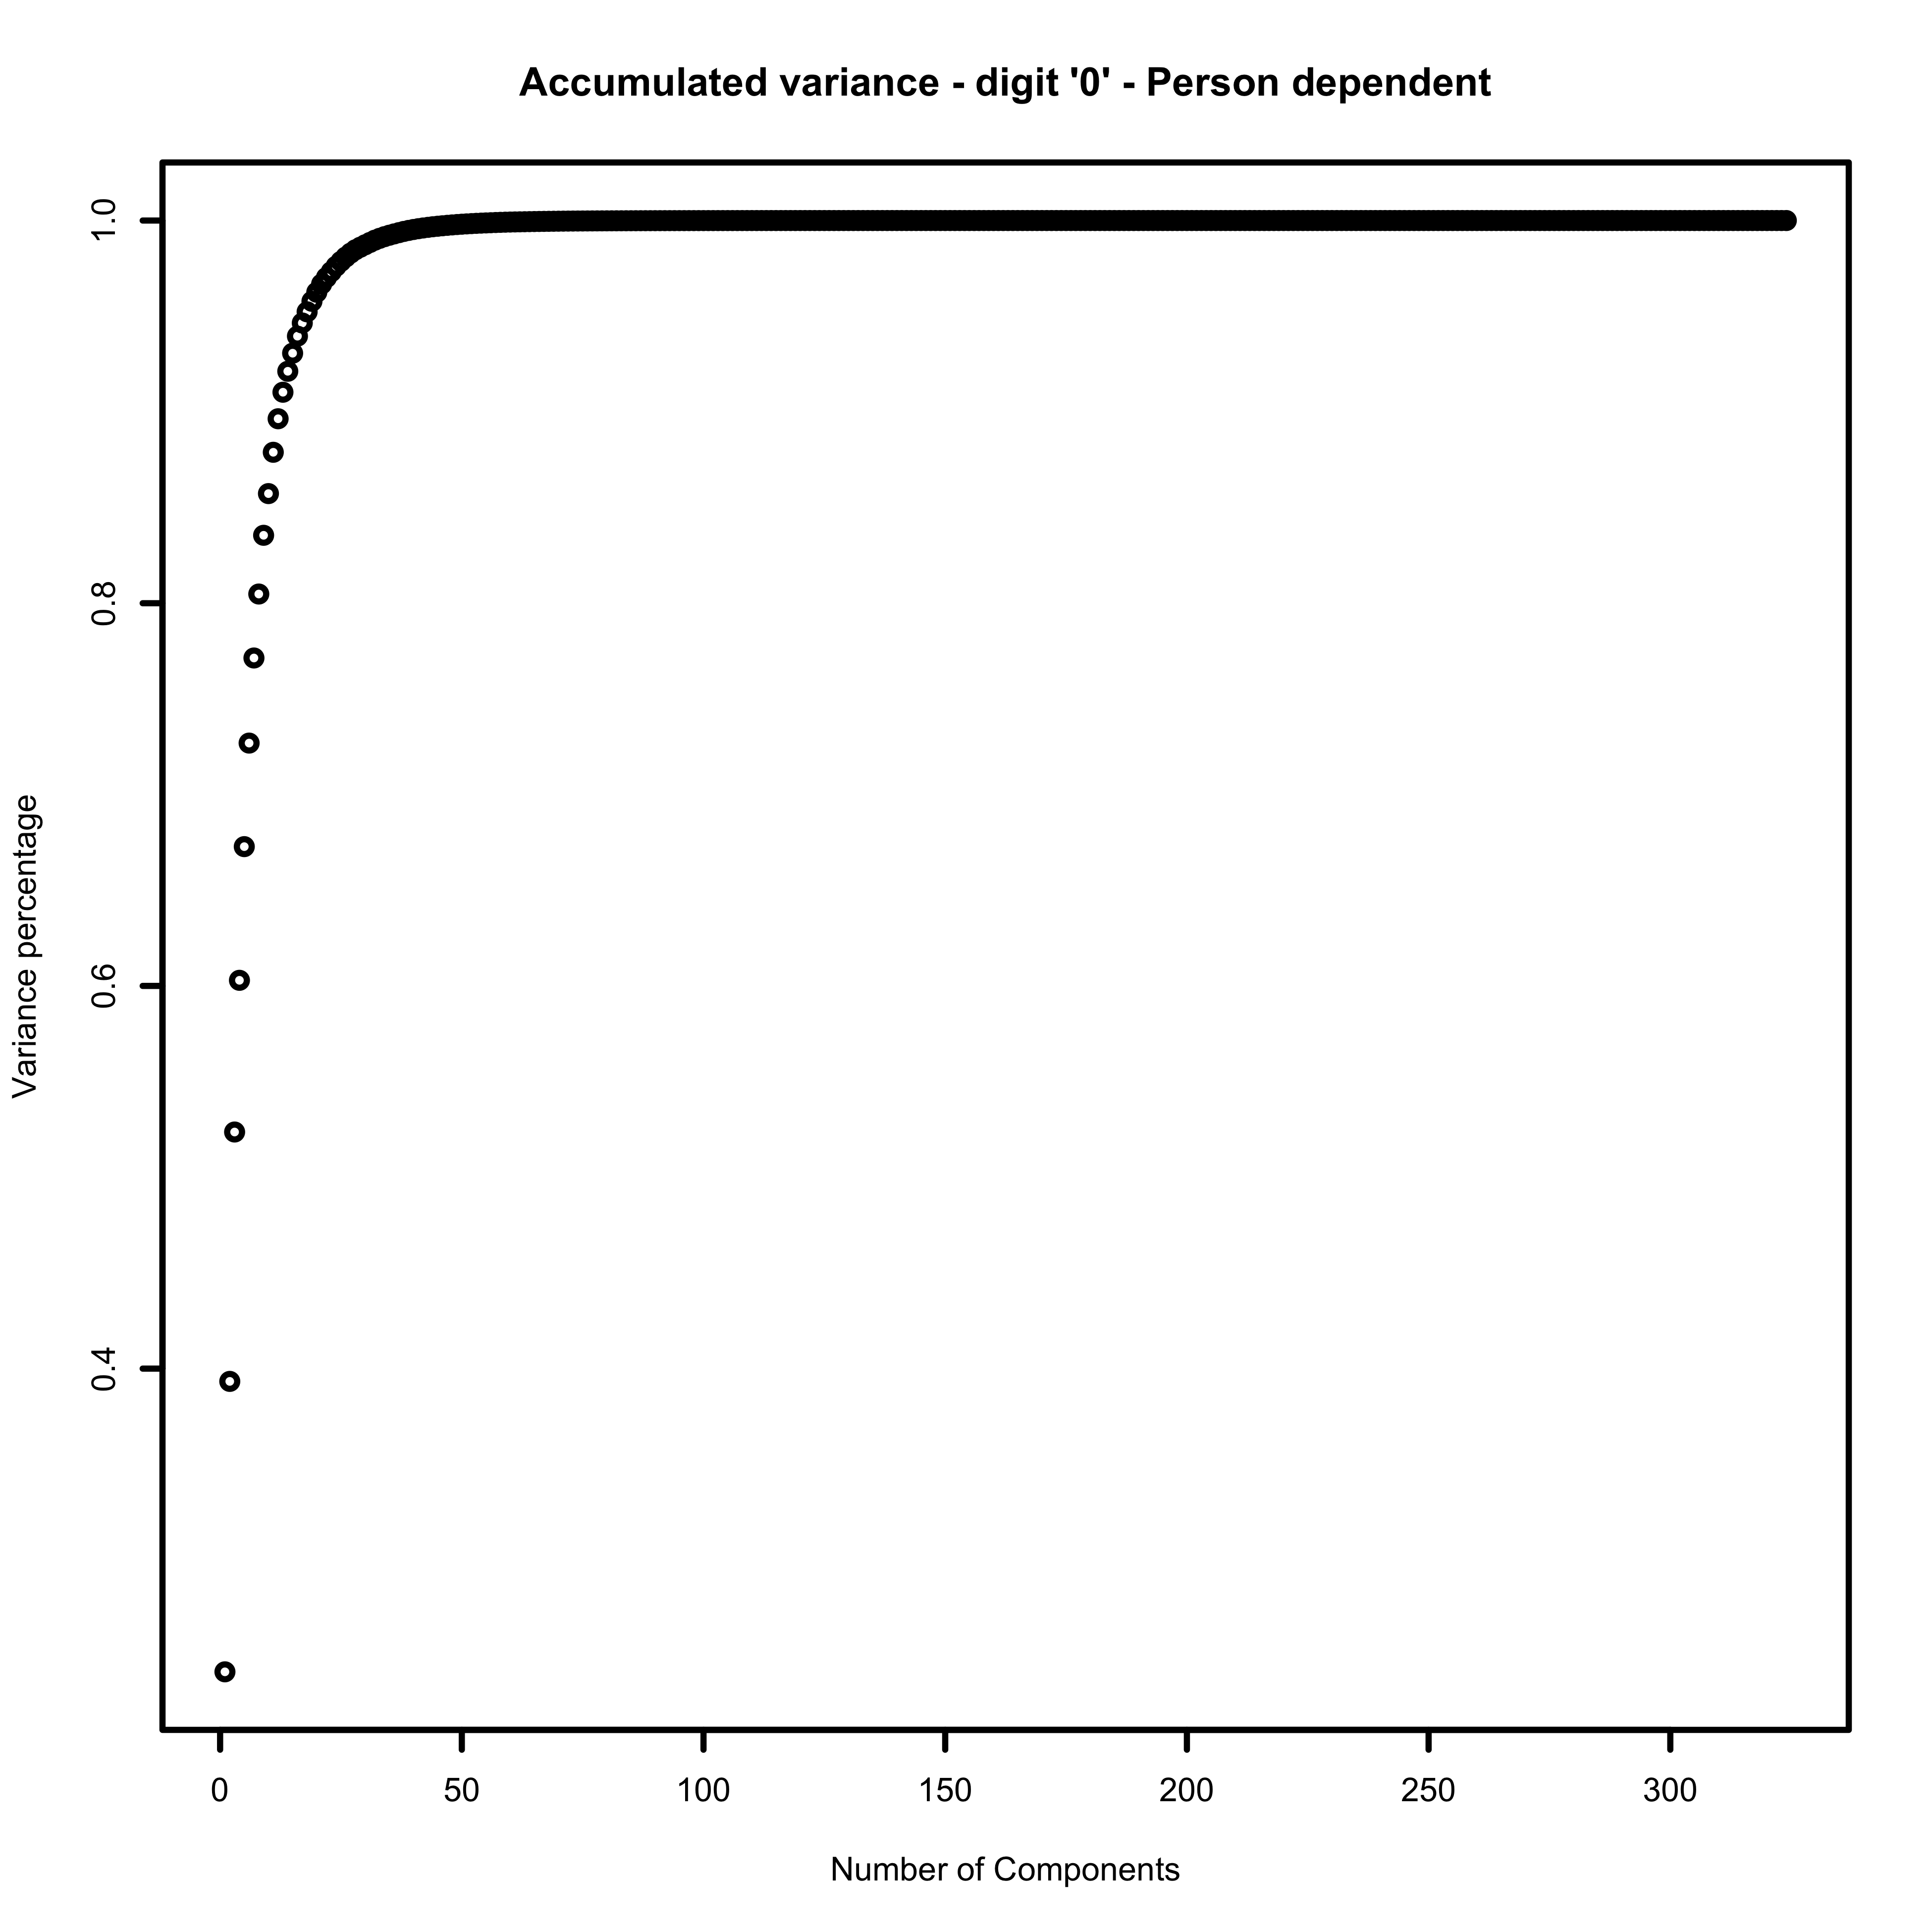
\includegraphics[width=1.7in]{Figure/accumulated-2-1-person-dependent.png}}%
  \hspace*{\fill}%
\end{figure}

\missingfigure{KnnFit plots}

The runtime for the training with the PCA components, has clearly been reduced compared to the training with the raw data. As the input data for training the system were reduced to PCA componentes. 

\missingfigure{knnFit trainingTime}
\todo[inline]{Insert PCA components needed for different trainings. }

\todo[inline]{prediction time.}